\section{Modelación}

La figura (\ref{fig:modcsinAWU}) muestra el sistema modelado en \textit{Simulink} sin 
considerar el efecto de \textit{Anti-Winding Up}. Este esquema permite observar el comportamiento del sistema 
cuando los actuadores alcanzan sus límites físicos, sin mitigar la acumulación del error integral.

\begin{figure}[H]
\centering
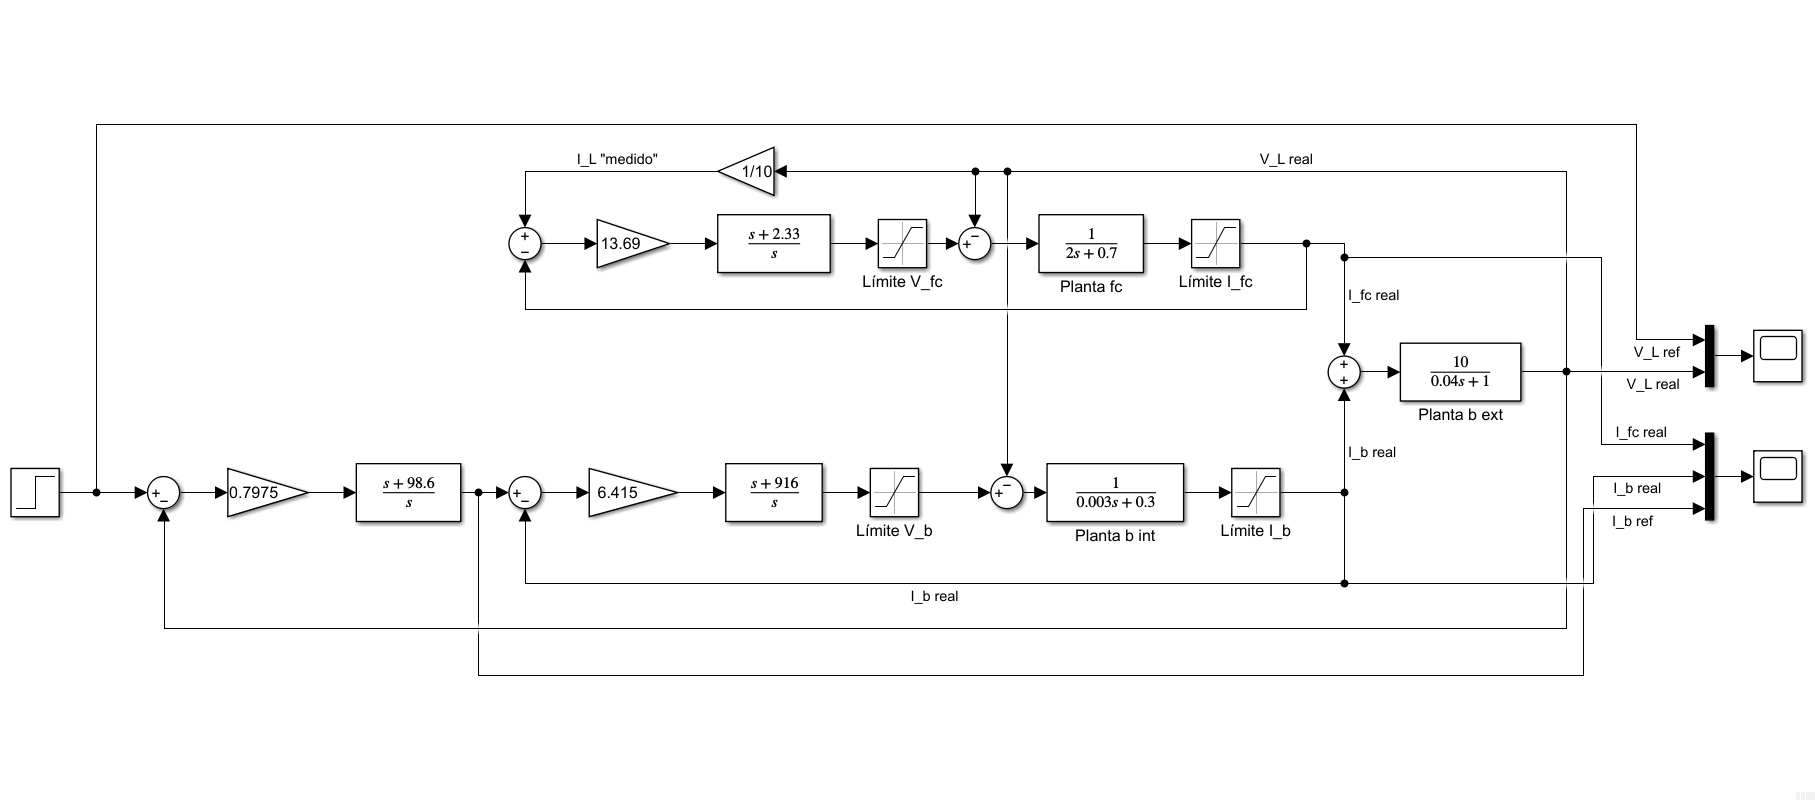
\includegraphics[trim={0 2.5cm 0 1cm},clip,width=1\linewidth]{img/modelacion/SistsinAWU.png}
\caption{Sistema sin considerar WindUp.}
\label{fig:modcsinAWU}
\end{figure}

En la figura (\ref{fig:modconAWU}) se muestra el mismo sistema, ahora con una estrategia 
de \textit{Anti-Winding Up} generalizado en los controladores asociados a plantas con restricciones físicas. 
Esta mejora busca evitar saturaciones prolongadas y optimizar la respuesta dinámica.

\begin{figure}[H]
\centering
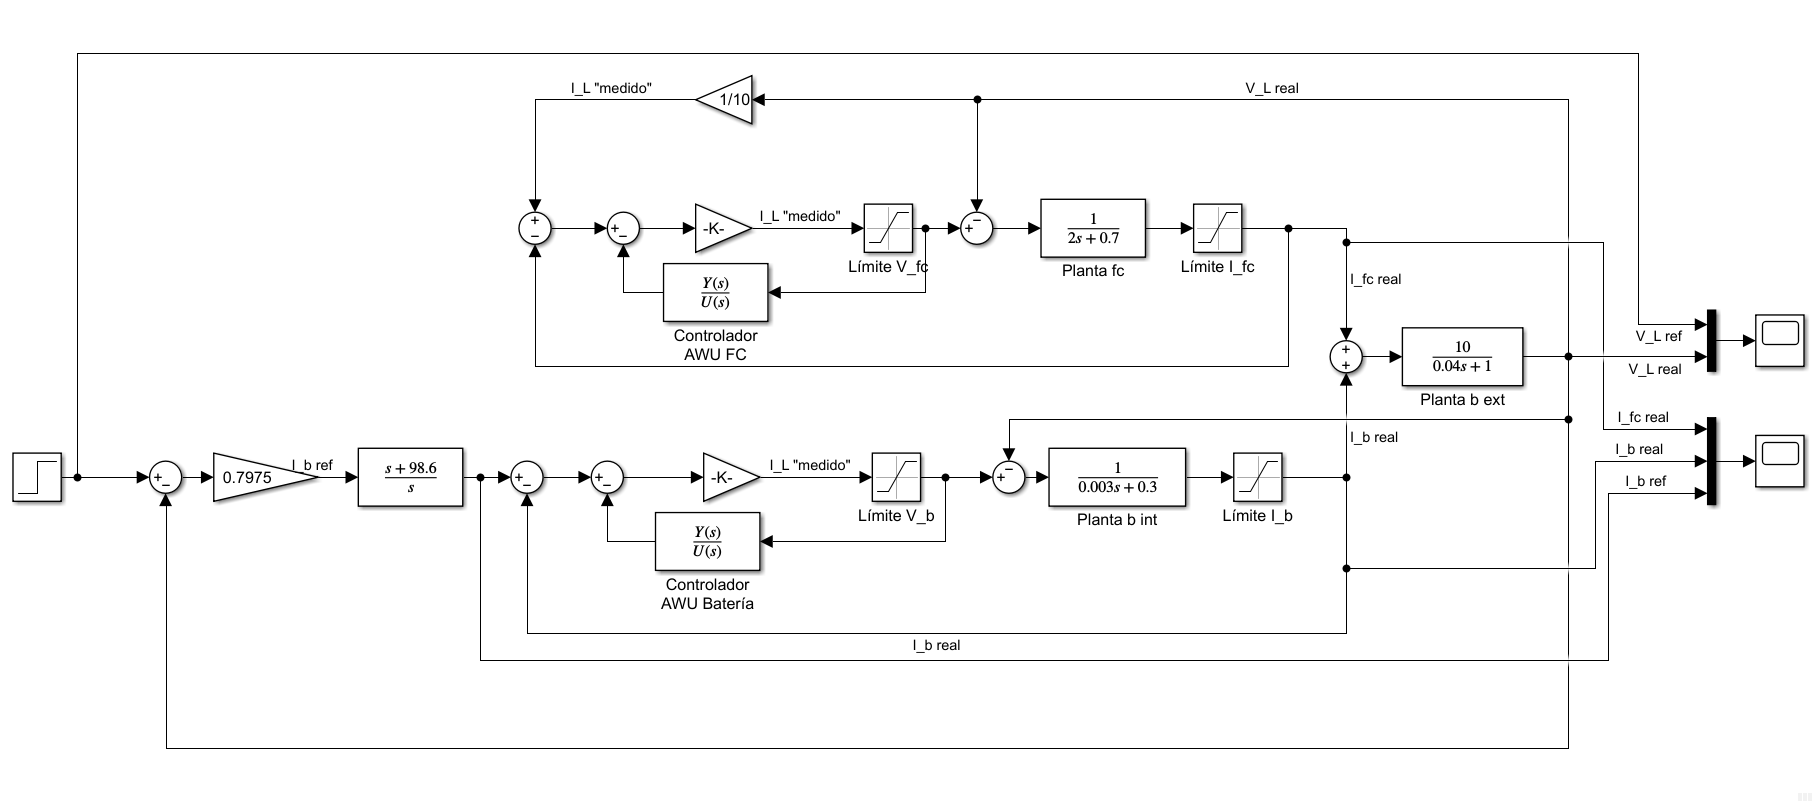
\includegraphics[width=1\linewidth]{img/modelacion/SistconAWU.png}
\caption{Sistema considerando WindUp.}
\label{fig:modconAWU}
\end{figure}
\newpage